\begin{figure*}[t]
    \centering
    \captionsetup[subfigure]{font=footnotesize}
    \begin{subfigure}[b]{0.32\linewidth}
        \centering
        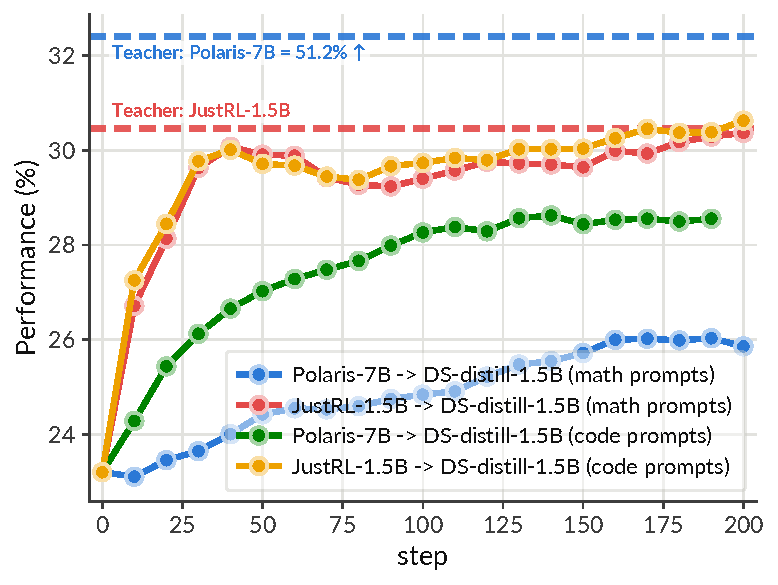
\includegraphics[width=\linewidth]{latex/figures/findings_2/1d5b_cross_domain_generalization_code_avg.pdf}
        \caption{LiveCodeBench (DS-distill-1.5B)}
        \label{fig:math_to_code_1d5b}
    \end{subfigure}
    \hfill
    \begin{subfigure}[b]{0.32\linewidth}
        \centering
        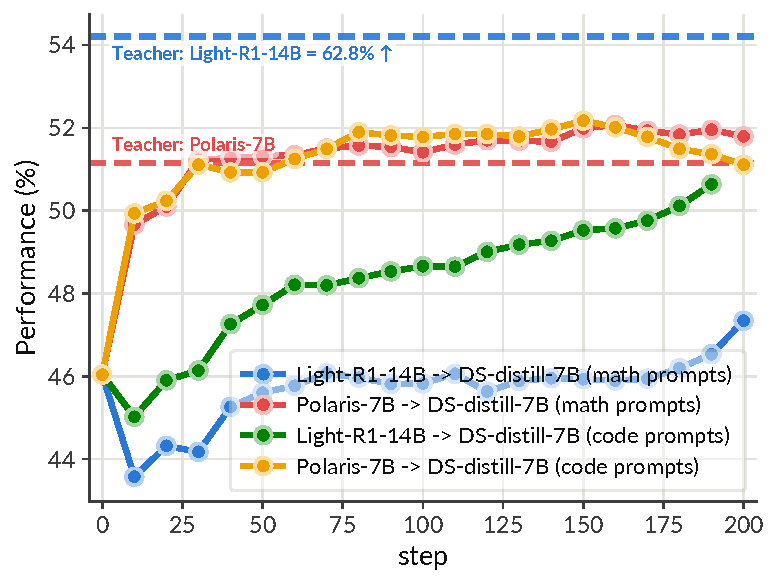
\includegraphics[width=\linewidth]{latex/figures/findings_2/7b_cross_domain_generalization_code_avg.pdf}
        \caption{LiveCodeBench（DS-distill-7B）}
        \label{fig:math_to_code_7b}
    \end{subfigure}
    \hfill
    \begin{subfigure}[b]{0.32\linewidth}
        \centering
        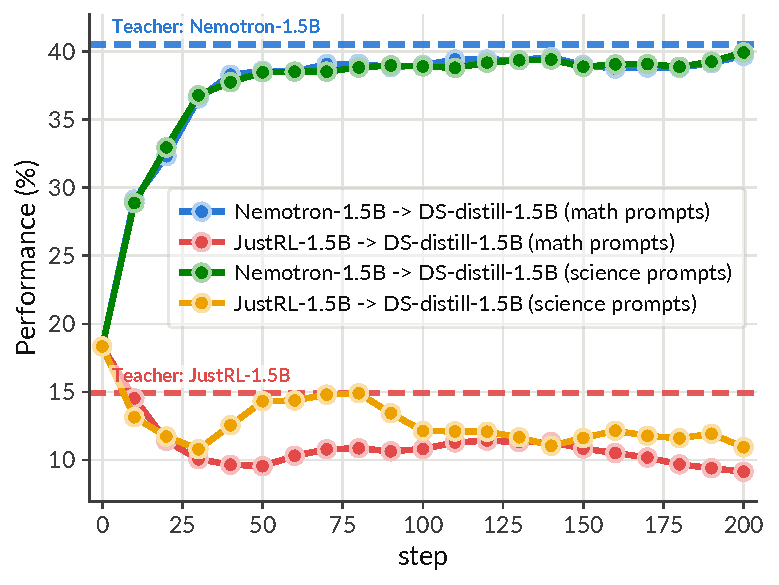
\includegraphics[width=\linewidth]{latex/figures/findings_2/1d5b_cross_domain_generalization_science_gpqa_avg.pdf}
        \caption{GPQA-钻石版（DS-精炼-1.5B）}
        \label{fig:math_to_science_1d5b}
    \end{subfigure}

     \begin{subfigure}[b]{0.99\linewidth}
        \centering
        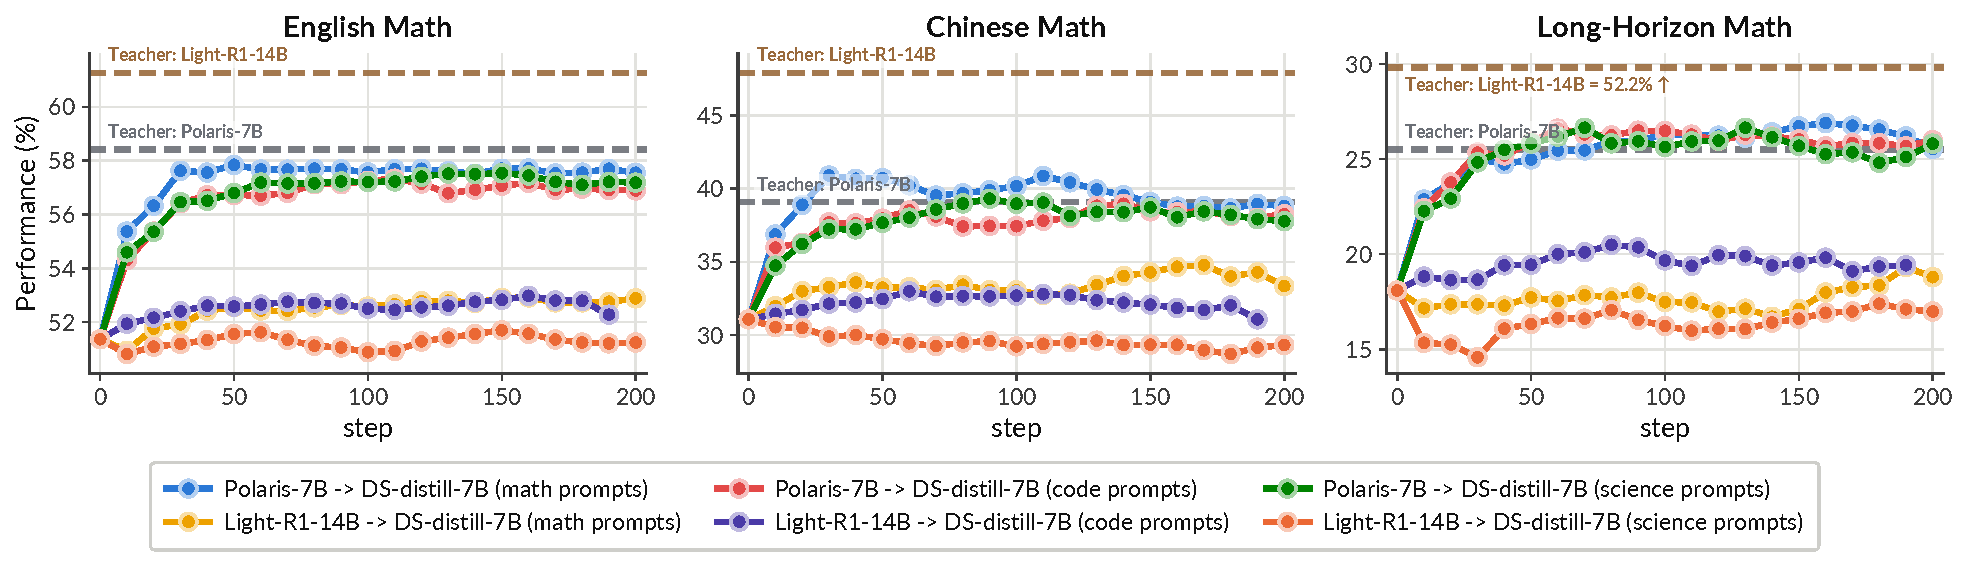
\includegraphics[width=\linewidth]{latex/figures/findings_2/7b_cross_domain_generalization_others_to_math_panel.pdf}
        \caption{在非数学领域进行训练，在数学领域进行评估（DS-distill-7B）}
        \label{fig:generalize_to_math_7b_panel}
    \end{subfigure}

    \caption{跨领域泛化在单教师OPD中的表现。对于同源OPD，基于数学提示进行训练时，学生在科学和代码任务上的表现也趋近于教师的表现，反之亦然。而对于跨源OPD，跨领域泛化性能显著下降：在(a)和(b)（LiveCodeBench评估结果）中，\textcolor{green!80!black}{绿色曲线}（基于代码提示训练）始终明显高于\textcolor{blue}{蓝色曲线}（基于数学提示训练）。虚线标记了教师单独训练的准确率。}
    \label{fig:cross_domain_generalization_math_to_others}
\end{figure*}
\section{跨领域泛化及其对多任务开放域问答的影响}
\label{sec:cross_domain}
我们现在转向跨领域泛化，即在某一领域的提示上执行OPD，并在其他领域上进行评估，以及其对MOPD的启示。本节提出两个相互关联的发现。首先，在同源OPD设置下，仅在某一领域的提示上进行训练，也能使学生在其他领域的表现接近教师的表现。相比之下，跨源设置中，跨领域泛化与域内泛化之间存在明显差距。因此，同源教师的影响并不局限于其训练提示所在的领域；在MOPD中将提示路由至不同领域的专家教师，并不能隔离它们的影响；调整教师混合比例会使得学生在各领域专家之间来回摆动，产生一种\emph{跷跷板效应}。
\subsection{OPD的跨领域泛化}
在跨领域泛化方面，我们研究了两个学生模型：DS-distill-1.5B 和 DS-distill-7B，并将每个学生模型分别与同源和跨源教师模型配对；例如，对于 DS-distill-1.5B，JustRL-1.5B 和 Nemotron-1.5B 是同源教师模型，而 Polaris-7B 是跨源教师模型。我们以两个方向运行 OPD：一是基于数学（教师模型强化学习后训练的领域）的提示进行训练，然后在代码和科学等其他领域进行评估；二是基于其他领域的提示（代码、科学和 IF）进行训练，然后在数学领域进行评估。
\paragraph{数学 $\rightarrow$  其他领域迁移。}
我们首先在数学提示上训练学生，然后在代码和科学任务上进行评估。如图~\ref{fig:math_to_code_1d5b} 和~\ref{fig:math_to_code_7b} 所示，尽管在OPD过程中未使用代码提示，但1.5B和7B的学生在LiveCodeBench上的得分均明显提升。科学任务上也出现了类似现象：如图~\ref{fig:math_to_science_1d5b} 所示，在数学和科学提示训练下，Nemotron-1.5B与JustRL-1.5B的表现对比显示了相同趋势。对于以科学为导向的Nemotron教师，经过数学或科学提示训练的学生最终达到相近的GPQA-Diamond得分水平，均显著高于初始学生得分。然而，由于以数学为导向的JustRL教师的科学推理能力弱于学生，因此无论采用数学还是科学提示进行训练，都会导致学生表现下降，最终使其GPQA得分低于初始水平。

\paragraph{其他领域 $\rightarrow$  数学迁移。}
如图~\ref{fig:generalize_to_math_7b_panel} 所示，使用代码或科学提示进行训练的学生在数学任务上表现提升（接近教师水平），且性能提升不仅限于英语，还扩展到中文和长时程数学基准。

这些结果表明，即使使用非主要领域的提示，教师的专长能力（即数学推理）也能传递给学生（见图~\ref{fig:if_to_math_cross_domain_generalization} 中的 IF$\rightarrow$ 数学迁移情况）。

综上所述，这些结果表明 \textbf{\emph{OPD 可以将能力从其训练提示的语义领域之外进行迁移：来自数学推理的监督信号能够引导学生在代码/科学推理能力上向教师靠拢，反之亦然}}。

\begin{insightbox}
\textbf{要点：}
OPD 可以在两个方向上将同一来源教师的能力从其训练提示的领域拓展出去：在数学提示上进行训练可提升学生在代码和科学方面的能力，而在代码、科学或指令遵循提示上进行训练则能反向提升数学能力，且提升效果延伸至中文和长序列数学问题。
\end{insightbox}

\paragraph{在OPD中，模型的泛化能力因模型来源而异。}
模型原点，首次出现在第~\ref{subsec:origin_indomain} 节，再次在跨领域情景中清晰显现。在图~\ref{fig:math_to_code_1d5b} 和~\ref{fig:math_to_code_7b} 中，同源教师在 LiveCodeBench 上对 \textcolor{yellow!85!black}{代码提示} 训练和 \textcolor{red}{数学提示} 训练均展现出一致的训练曲线：两者均 \textbf{趋近于} 教师的表现，因此在同源 OPD 情景下，训练领域差距基本消除，学生即使仅从数学轨迹中也能吸收教师的代码能力。

而跨源 OPD 的表现则截然不同：直接在目标领域进行训练仍为最优，我们观察到在领域内泛化（使用 \textcolor{green!80!black}{代码提示} 训练）与跨领域泛化（使用 \textcolor{blue}{数学提示} 训练）之间存在 \textbf{明显差距}。

我们将这一差异归因于教师与学生之间的分布差距。对于一个 \textit{\underline{同源教师}}，其输出分布相较于学生仅经过微调~\citep{yue2025does}，\textbf{\emph{OPD 在策略层面而非仅在训练领域上使学生与教师对齐}}。然而，对于一个 \emph{\underline{跨源教师}}，更大的分布差距使得这种对齐更加困难，\textbf{\textit{OPD 主要将学生策略拉向教师策略，且仅限于训练提示所覆盖的分布范围}}，导致跨领域泛化能力弱于领域内泛化。

\begin{insightbox}
\textbf{要点：}
跨领域迁移的范围受到模型原点的影响。同源教师模型（其分布与学生模型接近）即使在提示仅来自单一领域的情况下，也能使学生模型在跨领域上达到接近教师模型的水平，有效缩小训练领域间的差距。而异源教师模型面对更大的分布差异，在训练分布上的表现有所提升，但其跨领域泛化能力明显低于其领域内泛化能力。 
\end{insightbox}
\begin{figure*}[t]
    \centering
    \begin{subfigure}[b]{0.99\linewidth}
        \centering
        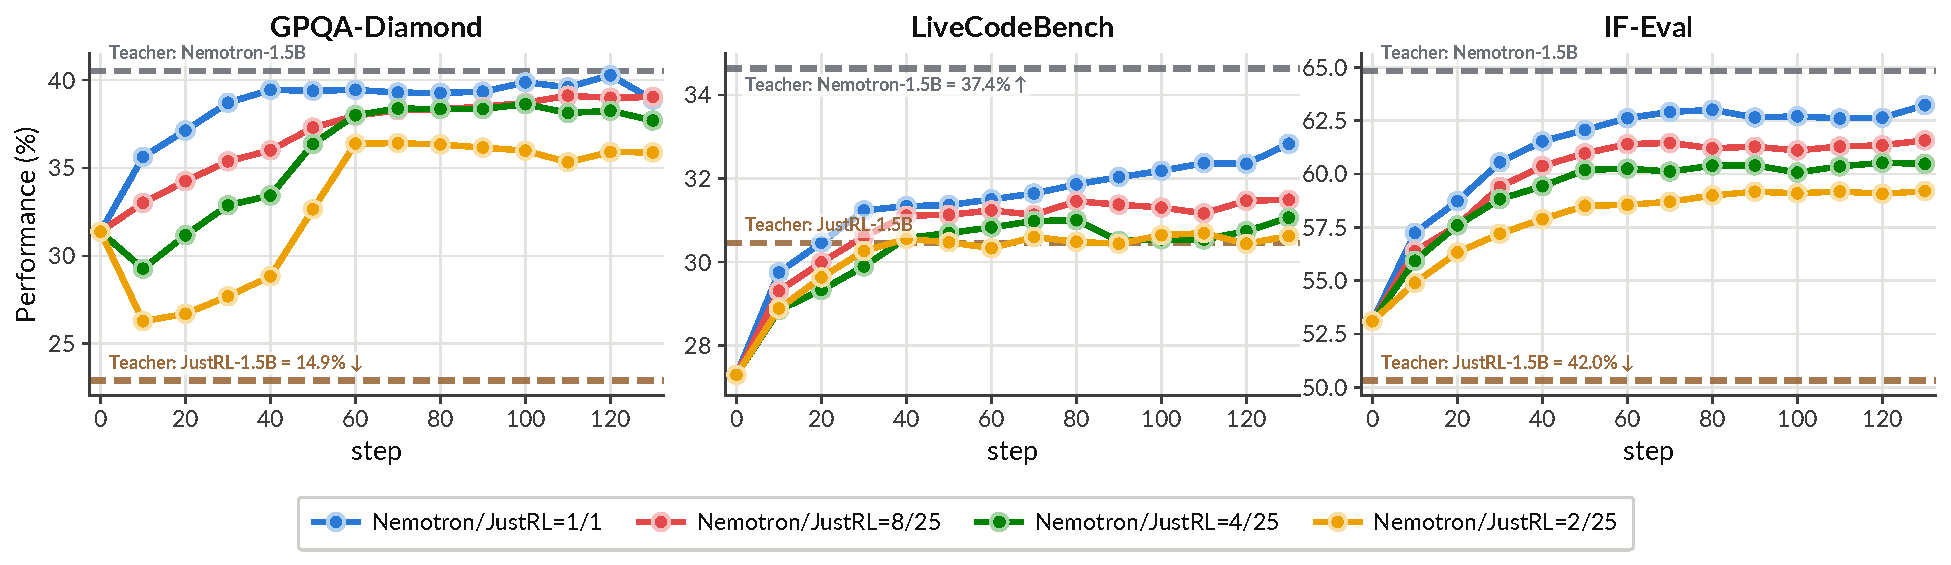
\includegraphics[width=\linewidth]{latex/figures/findings_3/mopd_nemo10step_panel.pdf}
        \caption{情景1. 数学老师：JustRL-1.5B；科学/如果老师：Nemotron-1.5B；学生：Dev-1.5B。}
        \label{fig:mopd_nemo10step}
    \end{subfigure}

    \begin{subfigure}[b]{0.99\linewidth}
        \centering
        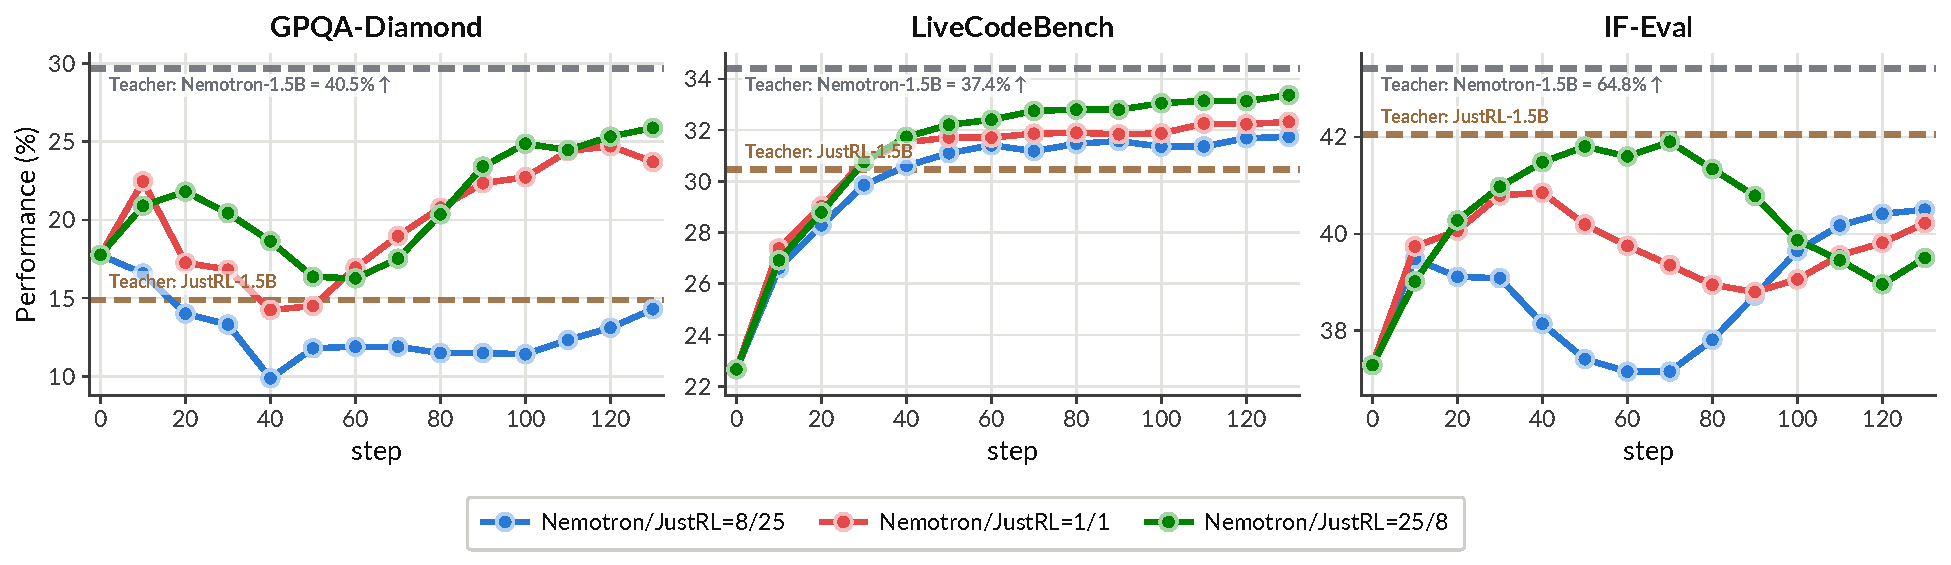
\includegraphics[width=\linewidth]{latex/figures/findings_3/mopd_reverse_teacher_panel.pdf}
        \caption{情景2. 数学老师：Nemotron-1.5B；科学/信息学老师：JustRL-1.5B；学生：DS-distill-1.5B。}
        \label{fig:mopd_reverse_teacher}
    \end{subfigure}

    \caption{\textbf{\emph{MOPD跷跷板效应}}。改变不同教师分配提示的混合比例，会显著影响OPD学生在不同领域的能力。例如，在子图(a)中，随着JustRL-1.5B（数学教师）数据比例的增加，学生的GPQA-Diamond（科学推理）、LiveCodeBench（代码推理）和IF-Eval（指令遵循）性能逐渐下降。}
    \label{fig:mopd_seesaw_effect}
\end{figure*}
\subsection{MOPD中的跨领域干扰}
\label{subsec:mopd}

\begin{table}[t]
\centering
\caption{不同JustRL-1.5B/Nemotron-1.5B混合比例（J/N）下的MOPD数学准确率。}
\label{tab:mopd-step200}
\resizebox{0.6\columnwidth}{!}{%
\begin{tabular}{c|cc|c}
\toprule
\textbf{Config} & \textbf{BeyondAIME} & \textbf{OlymMATH} & \textbf{Average} \\
\midrule
\midrule
DS-distill-1.5B & $9.6\%$ & $14.2\%$ & $11.9\%${\footnotesize \textcolor{black!60!black}{(\textbf{student})}} \\
\midrule
\midrule
\multicolumn{4}{c}{\textbf{\textit{Math Teacher: JustRL-1.5B, Science/IF Teacher: Nemotron-1.5B}}} \\
\midrule
$\mathbf{\text{J}/\text{N}=25/2}$ & $19.4\%$ & $33.3\%$ & $26.4\%${\footnotesize \textcolor{green!60!black}{(\textbf{+0.1 pp})}} \\
$\mathbf{\text{J}/\text{N}=25/8}$ & $19.6\%$ & $34.5\%$ & $27.1\%${\footnotesize \textcolor{green!60!black}{(\textbf{+0.8 pp})}} \\
$\mathbf{\text{J}/\text{N}=1/1}$ & $20.2\%$ & $32.4\%$ & $26.3\%${\footnotesize \textcolor{black!60!black}{(\textbf{baseline})}} \\
$\mathbf{\text{J}/\text{N}=8/25}$ & $19.7\%$ & $32.5\%$ & $26.1\%${\footnotesize \textcolor{red!60!black}{(\textbf{-0.2 pp})}} \\
$\mathbf{\text{J}/\text{N}=2/25}$ & $19.2\%$ & $31.0\%$ & $25.1\%${\footnotesize \textcolor{red!60!black}{(\textbf{-1.2 pp})}} \\
\midrule
\midrule
\multicolumn{4}{c}{\textbf{\textit{Math Teacher: Nemotron-1.5B, Science/IF Teacher: JustRL-1.5B}}} \\
\midrule
$\mathbf{\text{J}/\text{N}=25/8}$ & $17.4\%$ & $28.0\%$ & $22.7\%${\footnotesize \textcolor{green!60!black}{(\textbf{+0.7 pp})}} \\
$\mathbf{\text{J}/\text{N}=1/1}$ & $17.3\%$ & $26.6\%$ & $22.0\%${\footnotesize \textcolor{black!60!black}{(\textbf{baseline})}} \\
$\mathbf{\text{J}/\text{N}=8/25}$  & $17.1\%$ & $26.2\%$ & $21.7\%${\footnotesize \textcolor{red!60!black}{(\textbf{-0.3 pp})}} \\
\bottomrule
\end{tabular}%
}
\end{table}

\begin{figure*}[t]
    \centering
    \captionsetup[subfigure]{font=scriptsize}
    \begin{subfigure}[b]{0.32\linewidth}
        \centering
        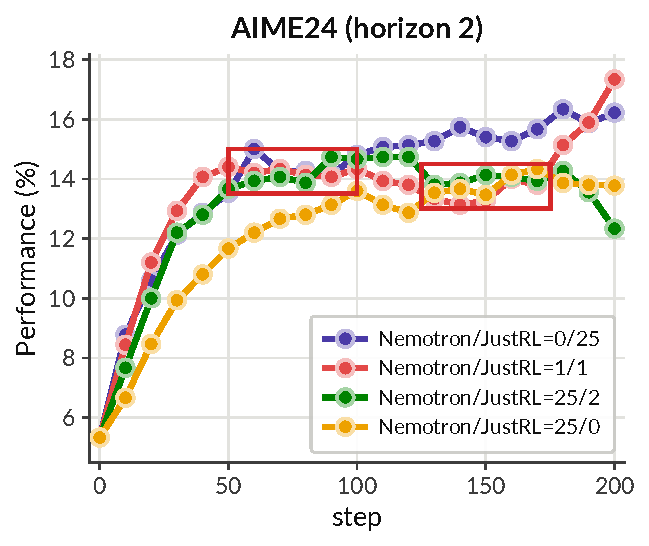
\includegraphics[width=\linewidth]{latex/figures/findings_3/mopd_forward_teacher_aime24_horizon2.pdf}
        \caption{JustRL-Math，Nemotron-Science/IF}
        \label{fig:switch_mopd}
    \end{subfigure}
    \hfill
    \begin{subfigure}[b]{0.32\linewidth}
        \centering
        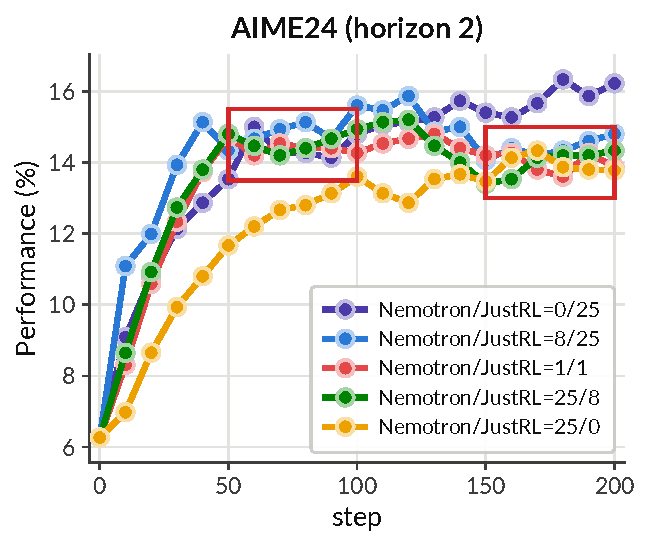
\includegraphics[width=\linewidth]{latex/figures/findings_3/mopd_reverse_teacher_aime24_horizon2.pdf}
        \caption{JustRL-Science/IF，Nemotron-Math}
        \label{fig:switch_mopd_reverse_teacher}
    \end{subfigure}
    \hfill
    \begin{subfigure}[b]{0.32\linewidth}
        \centering
        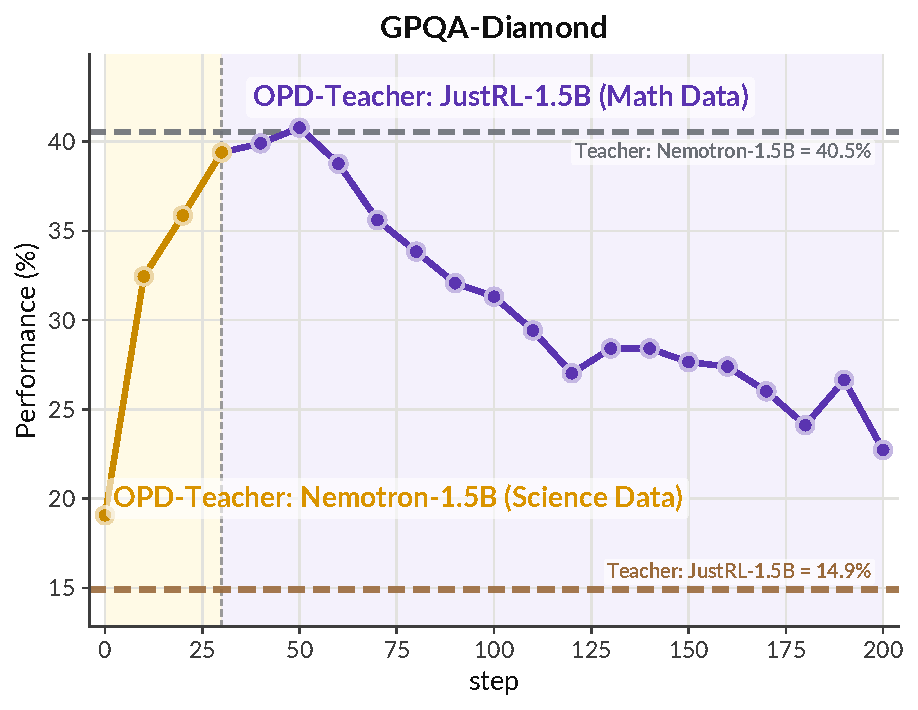
\includegraphics[width=\linewidth]{latex/figures/findings_3/mopd_teacher_switch_gpqa.pdf}
        \caption{级联OPD，GPQA-钻石}
        \label{fig:cascaded_opd}
    \end{subfigure}
    \caption{在MOPD训练过程中，教师之间的拉锯战可以被观察到。(a,b) \textcolor{red}{用红色框标出} 的部分显示，在两种情景下，MOPD学生的性能首先\textbf{\emph{跟踪}} \textcolor{violet}{仅使用JustRL的训练曲线}，随后逐渐向 \textcolor{yellow!85!black}{仅使用Nemotron的训练曲线} 偏移。(c) 在级联式OPD（先一个教师再另一个教师）中，受科学提示引导的Nemotron-1.5B指导时，GPQA性能 \textcolor{yellow!85!black}{急剧上升}，随后在数学提示引导的后续JustRL-1.5B作用下 \textcolor{violet}{回落}，从而在时间维度上解耦了多教师的影响。}
    \label{fig:additional_result_mopd}
\end{figure*}

单教师跨领域泛化观察对多教师开放领域推理（MOPD）具有关键但容易被忽视的含义：由于一个教师的影响范围远超其OPD训练提示所覆盖的领域，因此\textbf{\emph{将每个提示路由到特定领域的教师，并不能将其影响限制在分配的领域内}}。这为MOPD提出了一个实际问题：分配给不同领域的教师是否\emph{\textbf{争夺相同的能力}}，因为每个教师的跨领域影响可能与其他教师在其指定领域内的监督产生重叠和冲突。我们通过两个学生进行测试，Dev-1.5B\footnote{请参阅附录~\ref{sec:appendix_model_lineage} 以获取详细说明} 以及 DS-distill-1.5B 和两位具有互补特点的教师模型：JustRL-1.5B（在数学方面更强）和 Nemotron-1.5B（在科学和IF方面强得多，但在数学方面较弱）。在情景~1中，JustRL-1.5B 作为数学教师，Nemotron-1.5B 作为科学/IF教师。为了隔离路由提示领域的影响，并进一步探究此消彼长效应，情景~2 交换了它们的角色，使用 Nemotron-1.5B 作为数学教师，JustRL-1.5B 作为科学/IF教师，并追踪学生在各领域的表现变化。

\paragraph{教师混合比例引发跷跷板效应。}
当我们改变分配给两位教师的提示比例，同时保持其总量不变时，学生在每个基准上的表现会趋向于获得更大份额的教师，而非由教师所负责的领域决定。  
在情景~1（图~\ref{fig:mopd_nemo10step}）中，随着 JustRL（数学教师）所占份额增加（Nemotron/JustRL 从 $1/1$ 变为 $2/25$），学生的 GPQA-Diamond、LiveCodeBench 和 IFEval 得分均下降，趋近于 JustRL 较低的得分；\textbf{\emph{在 GPQA-Diamond 上，数学教师 JustRL 的拉力足够强，以至于准确率甚至在训练初期就下降了 $\sim5\%$ }}，因为 JustRL 在该指标上的得分低于学生 Dev-1.5B。在情景~2（图~\ref{fig:mopd_reverse_teacher}）中，当 Nemotron 被指定为数学教师时，同样的三个基准得分随 Nemotron 份额增加而上升，向 Nemotron 在这些基准上更高的得分靠拢。  
数学领域的结果（表~\ref{tab:mopd-step200}）给出了相反的情况：适当提高 JustRL 的份额（因其数学表现优于 Nemotron）能提升数学得分，无论其被分配到哪个领域。

最终，性能的转变不仅仅由教师指定的领域决定：\textbf{\emph{均匀增加教师的占比会将多领域能力拉向该教师的基准水平，形成一种依赖混合比例的跷跷板效应，使得针对特定领域的提示路由无法有效限制教师的影响}}。


\paragraph{训练期间可以观察到教师之间的一场拔河较量。}
最后，教师之间的平衡在训练过程中发生变化。在 AIME24-Horizon-2 的两种情景下（图~\ref{fig:switch_mopd} 和~\ref{fig:switch_mopd_reverse_teacher}），MOPD 学生最初跟随更强数学能力的 JustRL-only 曲线，随后逐渐偏离并趋向于更低的 Nemotron-only 水平，因此学生并未立即稳定在某个固定的混合结果上，而是随着训练的进行在两个教师之间不断被拉扯。

在图~\ref{fig:switch_mopd} 中，当 JustRL 作为数学教师时，我们可以观察到，最终红色曲线（Nemotron/JustRL 混合比例 $1/1$）重新被拉回至 JustRL-only 曲线，而黄色曲线（Nemotron/JustRL 混合比例 $25/2$，分配给 JustRL 的提示更少）则完全被拉向 Nemotron-only 曲线。

此外，我们还开展了一项级联 OPD 实验（图~\ref{fig:cascaded_opd}），以在时间维度上解耦多教师 OPD 训练的影响：首先使用科学能力更强的 Nemotron-1.5B 教师和科学提示进行训练，使 GPQA 提升至其水平；在切换为 JustRL-1.5B 教师和数学提示后，GPQA 又回落至原始水平。


\paragraph{跷跷板效应为分析MOPD提供了一个心理模型。}
跷跷板效应为分析MOPD~\citep{chen2026counteraction}中的抵消作用提供了一个有用的视角：当学生在某一领域表现不佳时，原因未必在于被分配至该领域的教师，因为另一名教师可通过其自身的跨领域迁移拉动相同的能力。这表明，在诊断MOPD时，应考察全部教师集合，而非仅关注所涉领域的领域专家；同时也表明，一名领域专家在其目标领域之外所具备的能力，与其在MOPD中的行为相关，而不仅限于其在所分配领域上的表现。因此，传统的提示路由范式~\citep{ma2026mopd,coreteam2026mimov2flashtechnicalreport,huang2026kat,xu2026deepseek}并不能保证不同领域专家的能力彼此隔离。

\begin{insightbox}
\textbf{要点：}
由于教师的影响不限于其OPD提示所在的领域，因此在多教师OPD（MOPD）中将提示路由给领域专家也无法将其完全隔离。随着混合比例的变化，学生在每个基准上的得分会趋向于占比更大的教师，且趋向于该教师自身的水平，而非其被分配到的领域水平。  
因此，结合专家会产生一种与混合比例相关的\emph{跷跷板}效应，而非专家技能的简单叠加。这一现象为诊断MOPD提供了有益视角：某一领域表现不佳，可能源于其他教师的跨领域影响，因此领域专家的非本领域行为同样重要。
\end{insightbox}
